\section{Passengers}

In this section the passengers of air traffic will be described. 

\subsection{Expectations}
In a survey made by eNT - Global Travel Industry News, they asked more than 3.200 people what they thought is the most important thing in their flight.
\begin{itemize}
  \item 25\% - thought limited legroom was one of their biggest gripes about air travel
  \item 30\% - lobbied for more legroom
  \item 38\% - requested roomier seats
  \item 25\% - consider airline fees to be their biggest complaint about air travel
  \item 56\% - thought checked baggage fees were the most annoying current airline fee
  \item 56\% - expect the overall cost of airline fees to rise in 2010
 \item 74\% - think passengers of size should be required to purchase tickets for two seats on their flights
  \item 21\% - think that airlines will add passenger of size fees in 2010
  \item 30\% - they would be more likely to book a flight on an aircraft with in-flight Wi-Fi than one without
  \item 61\% - they would not be willing to pay for in-flight Wi-Fi access
  \item 27\% - they would be willing to pay \$5 or less for the service
\end{itemize}
With the rise of checked baggage fees:
\begin{itemize}
 \item 58\% - said they always or often carry on their bag to avoid extra charges, possibly adding to cramped overhead bins
 \item 62\% - said they would put their carry-on bag above someone else's row if their own overhead space were already filled
 \item 57\% - said that each seat on a plane should have assigned space in the overhead compartment, even if it meant carry-on bags had to be smaller
\end{itemize}

\subsection{Information}
Passengers want control over and knowledge about their journey on the run. The number of passengers who has a smartphone went from 54\% in 2011 to 70\% in 2012 and is expected to reach 90\% in 2015. Therefore it it clear that the market for smartphone applications for the passengers witch can keep them informed about their flights, delays, boarding hours etc. and which they can also use to check-in and acquire their boarding passes. Already 21\% of passengers are now using mobile boarding pass.
Another survey made by IATA in 2012 shows that only a very small procentage uses the Airline application for smartphones to book their flight whereas 52\% books online via the airline website, see figure \ref{channes used to book}.

\begin{figure}
\centering
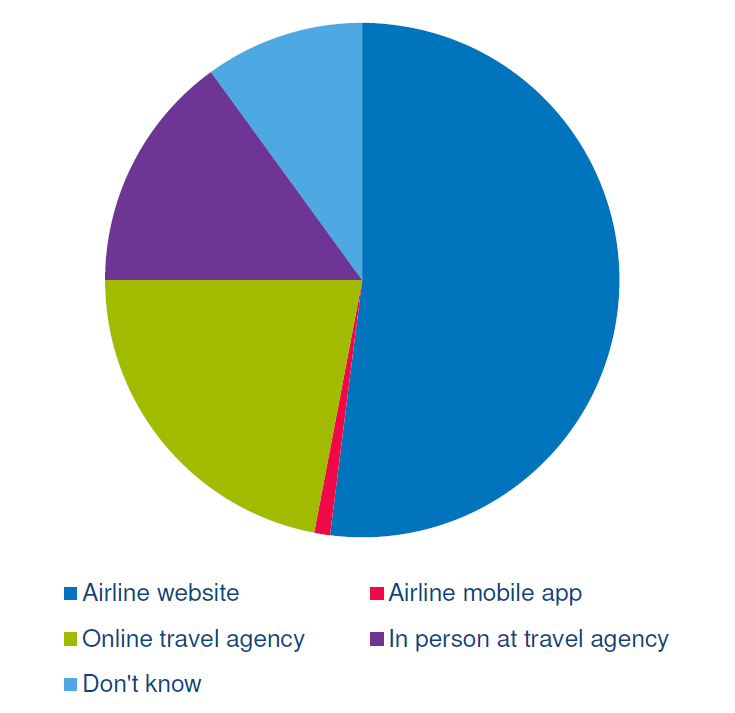
\includegraphics{Grafik/channes_used_to_book}
\caption{Breakdown of channels used to book flights.}
\label{channes used to book}
\end{figure}


In conclusion the passengers have different expectations for the flight companies, and it will not be easy to satisfy every customer fully. To do so would be a major challenge, but also one that might raise the number of people challenging???????Hvad menes der????? with the air traffic. But for ground handling companies passengers is no concern to them, other than check-ins and take-off schedules.

%Kilder:
%http://www.iata.org/publications/Documents/2012-iata-global-passenger-survey-highlights.pdf
%http://business.time.com/2012/09/20/airline-introduces-perk-passengers-actually-want-and-its-free/
%http://consumertravelalliance.org/2011/02/06/what-do-airline-passengers-really-want-%E2%80%94-besides-a-good-fare/
%http://www.eturbonews.com/14902/survey-what-passengers-want-airlines
%http://elliott.org/blog/what-do-airline-passengers-really-want-besides-a-good-fare/
%http://blog.apex.aero/inflight-services-2/ten-premium-passengers-airlines/

